% --- SLIDES : Challenge 1 ---

\section{Challenge Diffie-Hellman}

\begin{frame}
    \frametitle{Diffie-Hellman : \textit{Man-in-the-middle | Export grade}}
    \framesubtitle{Objectifs}
    \begin{center}
        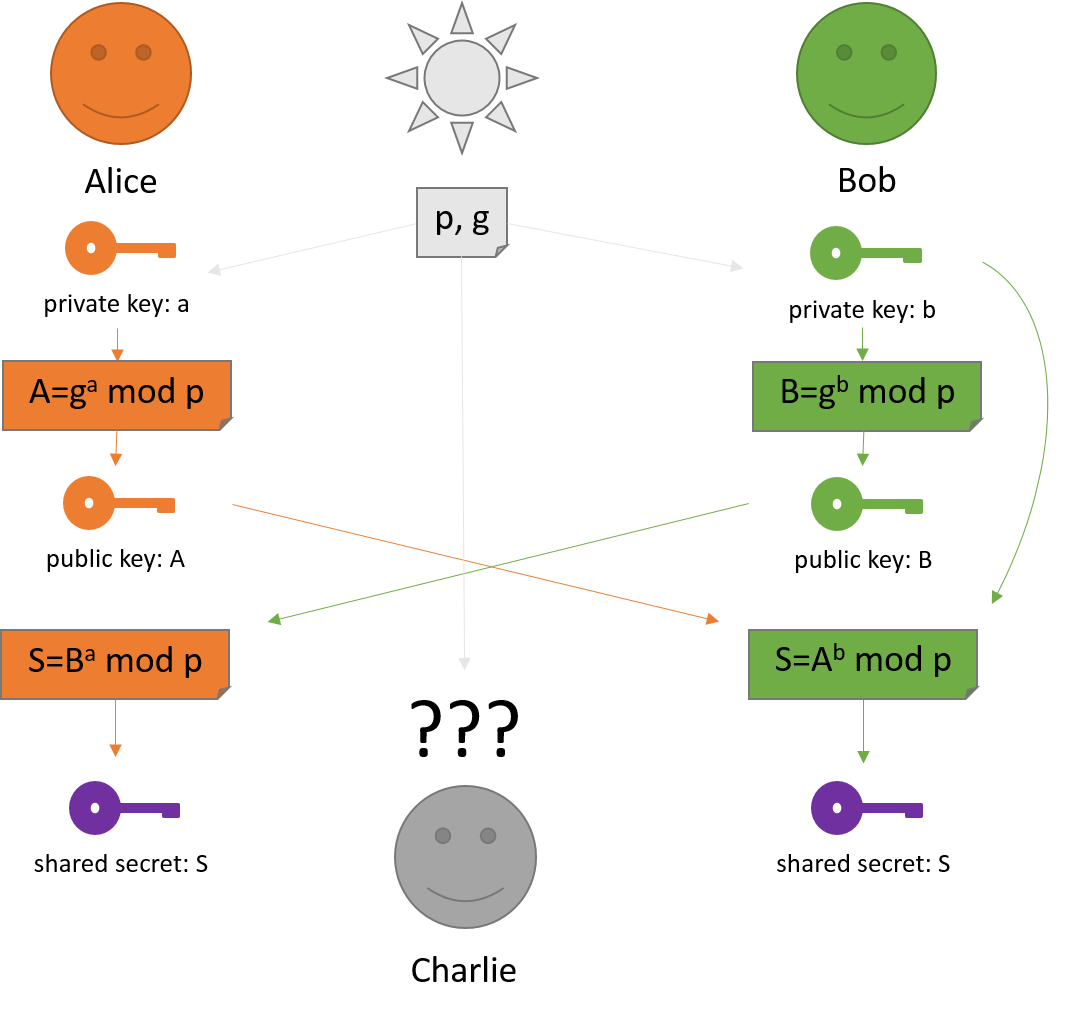
\includegraphics[width=0.65\textwidth]{Images/diffie_key_exchange.png}
        \vspace{0.5em}

        {\small\itshape Schéma : attaque Man-in-the-Middle exploitant des suites export-grade}
    \end{center}
\end{frame}

\begin{frame}
    \frametitle{Diffie-Hellman : \textit{Man-in-the-middle | Export grade}}
    \framesubtitle{Méthode de résolution}
    \begin{itemize}
        \item Quel est le but ?
        \item Quelle vulnérabilité est exploitée ?
    \end{itemize}
\end{frame}


\begin{frame}
    \frametitle{Diffie-Hellman : \textit{Man-in-the-middle | Export grade}}
    \framesubtitle{Résultat}
    \begin{itemize}
        \item Quel est le but ?
        \item Quelle vulnérabilité est exploitée ?
    \end{itemize}
\end{frame}